As mentioned in the Methodology section~\ref{sec:methodology}, the first step was to analyse time series of the anemometers and thermocouples averaged in a 30 minute period. 

The top panel of figure~\ref{fig:temp_series} shows the CSAT3 air temperature and the ground temperature measurements. At first glance is possible to see that there is a gap in the data between the 17th and the 19th of February when none of the CSAT3 instruments were measuring. In the lower panel, we can see the time series of the Thermocouples. They follow a similar variation as the CSAT3 instruments, but they were recording during the whole campaign. 

\begin{sidewaysfigure}
  \centering
  {
  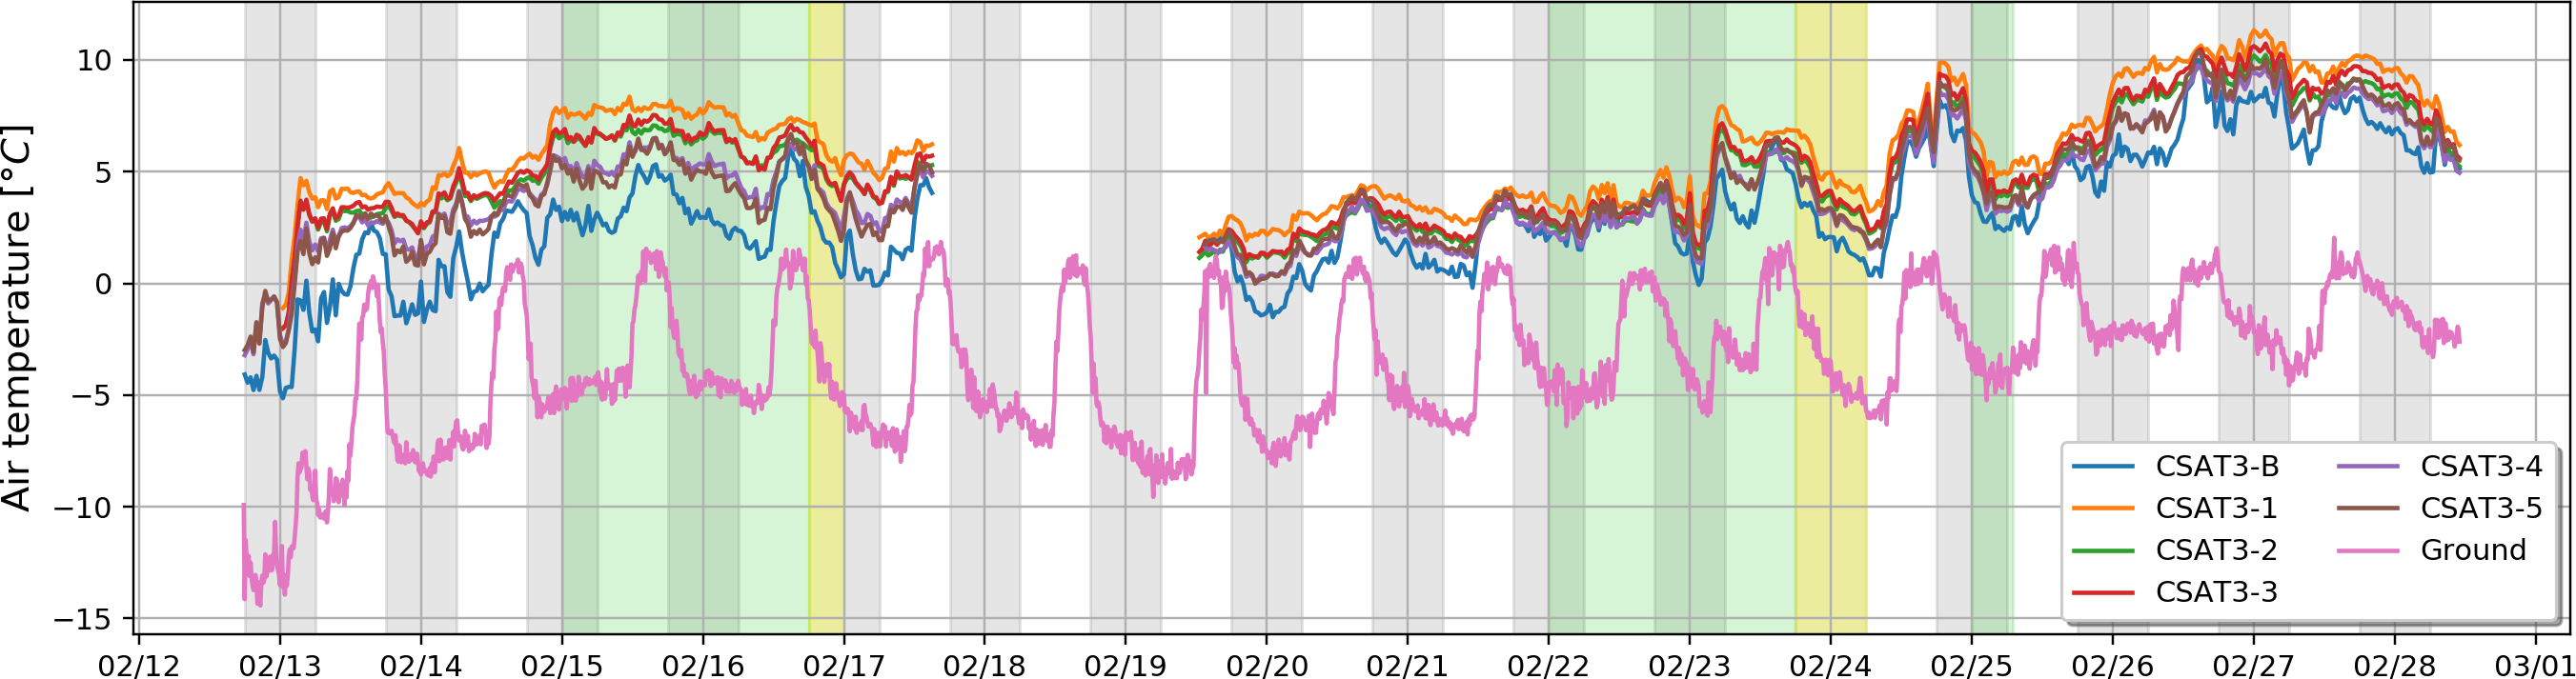
\includegraphics[width=1\textwidth]{fig/chapter_4/csat_temp_series.png}\\
   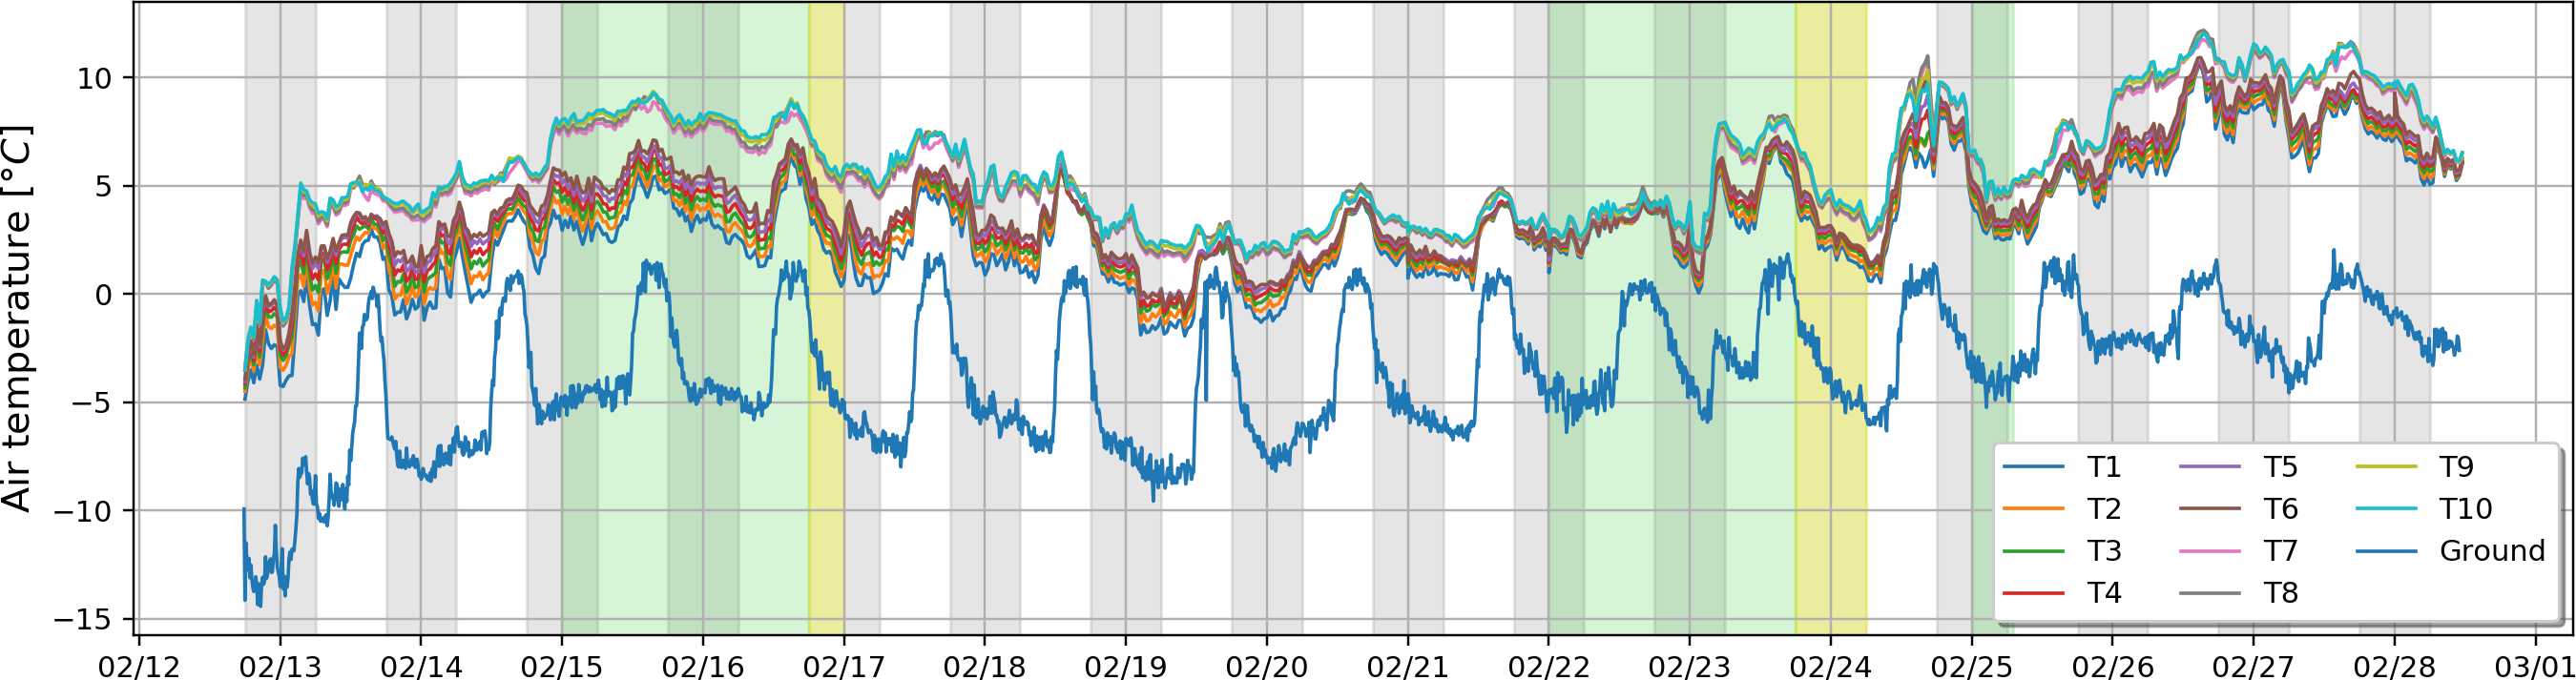
\includegraphics[width=1\textwidth]{fig/chapter_4/TC_temp_series.png}
   }
  \caption{Time series of air temperature of the whole field campaign. The top panel shows the air temperature recorded by the CSAT3 instruments and the lower panel the air temperature recorded with the Thermocouples. In both figures, the grey shadows represent the night periods, the green shadows the favourable days from in situ observation and the yellow shadows the nights chosen for the analysis. Both plots have the ground temperature as a reference point.}
  \label{fig:temp_series}
\end{sidewaysfigure}

In figure~\ref{fig:windspeed_series} the time series (30 minutes average) of the wind speed of the CSAT3 and the Windsonic anemometers are shown. The top panel corresponds to the CSAT3's, where is possible to see the gap of the data in the middle of the campaign. The lower panel corresponds to the Windsonic 2-D instruments, where we can see that during the beginning of the campaign (from the 12th to the 19th) only the Winsonic No.0 and No.1 were working. From the 19th until the end of the campaign, the four Windosinc were working. 

\begin{sidewaysfigure}
  \centering
  {
  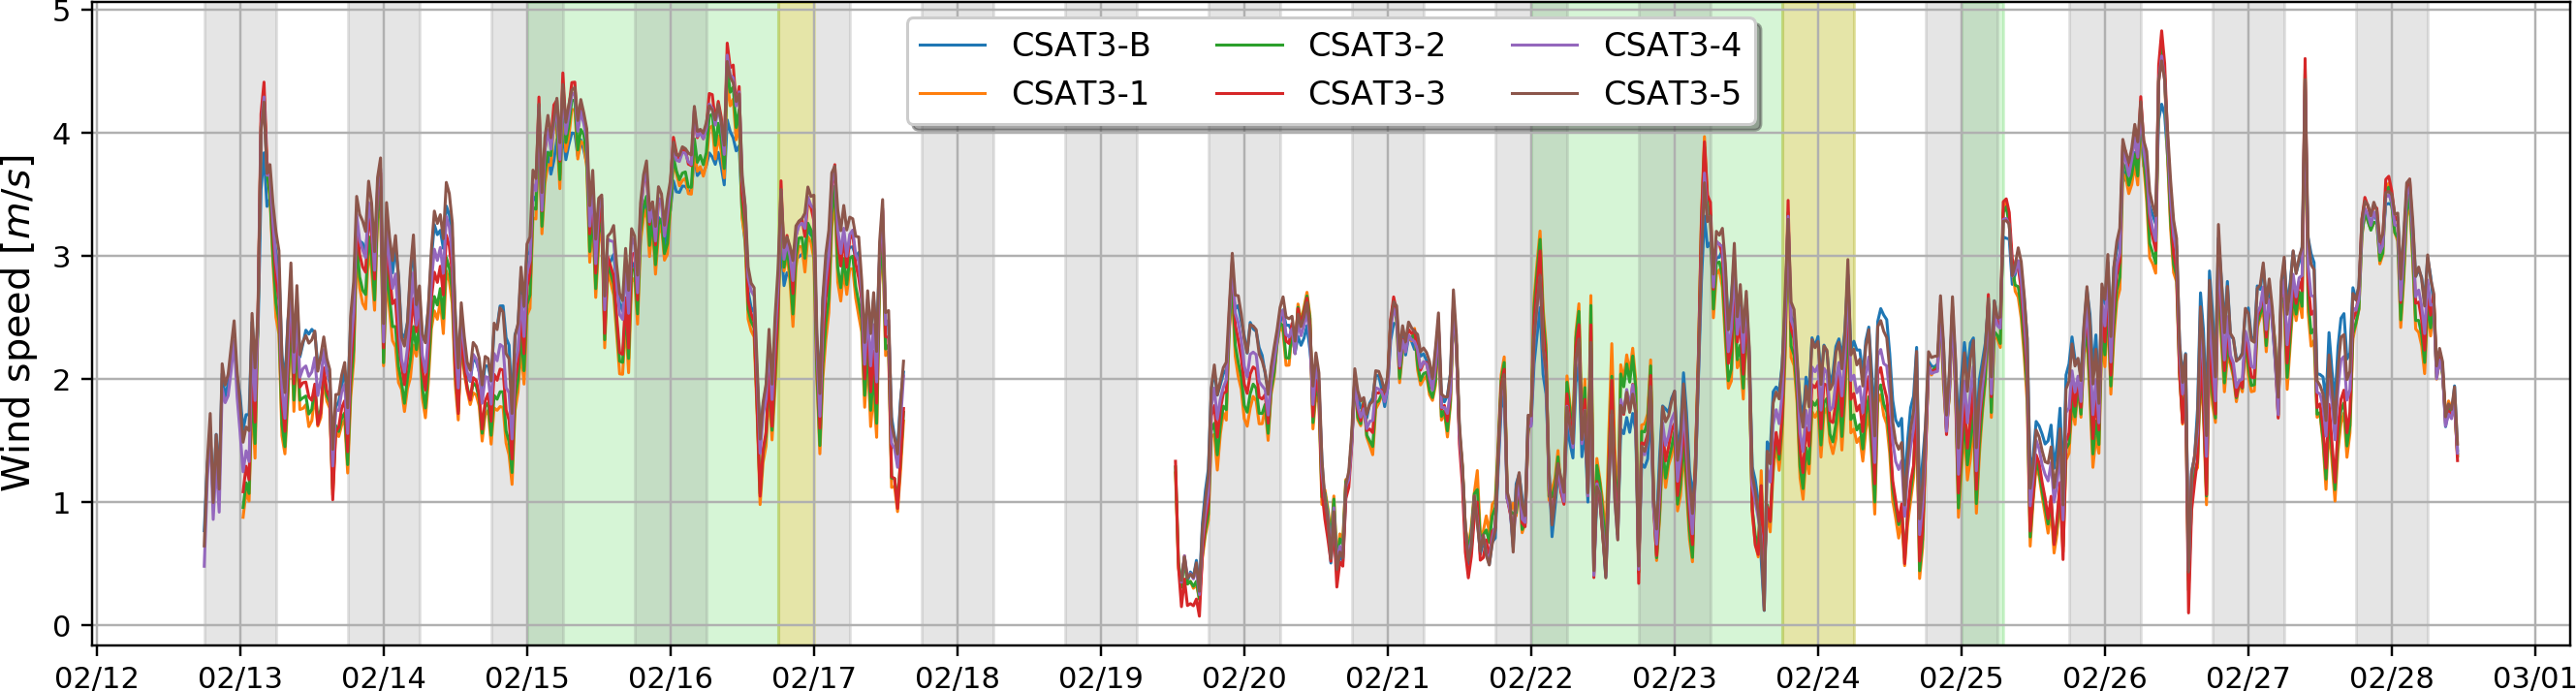
\includegraphics[width=1\textwidth]{fig/chapter_4/wind_speed_csat_series.png} \\
   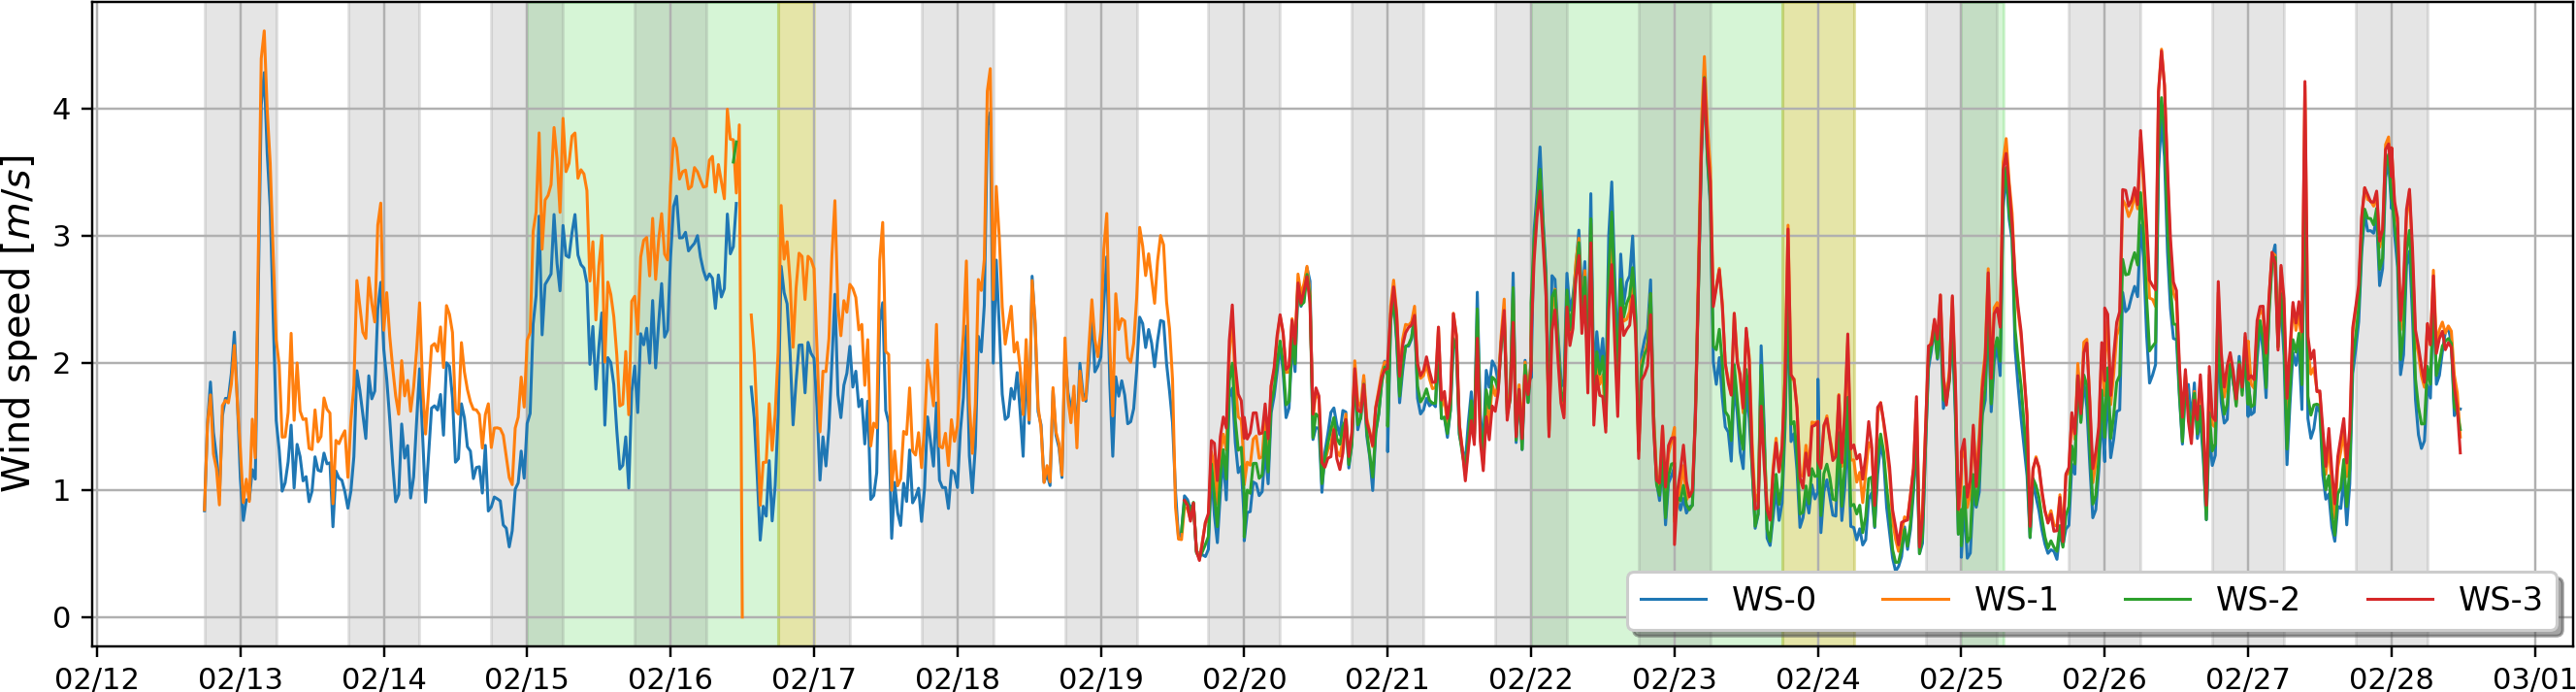
\includegraphics[width=1\textwidth]{fig/chapter_4/wind_speed_ws_series.png}
   }
  \caption{Time series of wind speed of the whole field campaign. The top panel shows the wind speed recorded by the CSAT3 instruments and the lower panel the winds speed recorded with the Windsonic 2-D (WS). In both figures, the grey shadows represent the night periods, the green shadows the favourable days from in situ observation and the yellow shadows the nights chosen for the analysis. Both plots have the ground temperature as a reference point.}
  \label{fig:windspeed_series}
\end{sidewaysfigure}

In both figures~\ref{fig:temp_series} and \ref{fig:windspeed_series}, there are periods marked by green and yellow shadows. The green ones indicate the favourable days for the development of katabatic winds, according to the in situ observations: cold nights with steady decrease of surface temperature during the night with weak wind. The yellow periods indicate the nights that were selected for the analysis in this work, according to the criteria for choosing a good night. We selected the nights of the 16th to the 17th and the night from the 23rd to the 24th. These were chosen because there was a pronounced drop in the temperature of the ground and the air and because they were in the favourable periods to detect these winds. 

For the 16-17th night, the instruments recorded a drop in the average temperature of more than $5\degree C$ for the ground temperature and air temperature, from the sunset until midnight. At midnight the instruments measured a small increase in the temperature of the air, which probably was caused by the presence of an external wind system. If we look at the wind speed profiles, on the same night, we can see that at the end of the afternoon the wind is relatively calm, and increases its intensity during the night. During the 23-24th night, the conditions were similar, with the exception that the ground and air temperature decreased very uniformly throughout that night.

\section{Calibration}

To corroborate that the measurements of temperature and wind speed done by different types of instruments where congruent between them, we performed some comparisons between the CSAT3's and the Thermocouples, for temperature, and the CSAT3's with the Windsonics, for the wind speed.

Figure~\ref{fig:csat1_vs_ws3} shows a scatter plot comparing 30 minutes averaged wind speed, measured with the Windsonic 2-D, versus the wind speed measured with the CSAT3-B. Using the data of the whole campaign, a linear regression was done, from which it was found a correlation coefficient $R = 0.94$. This means that both wind speeds are correlated and their variation in time is similar. 

\begin{figure}[!ht]
    \centering
    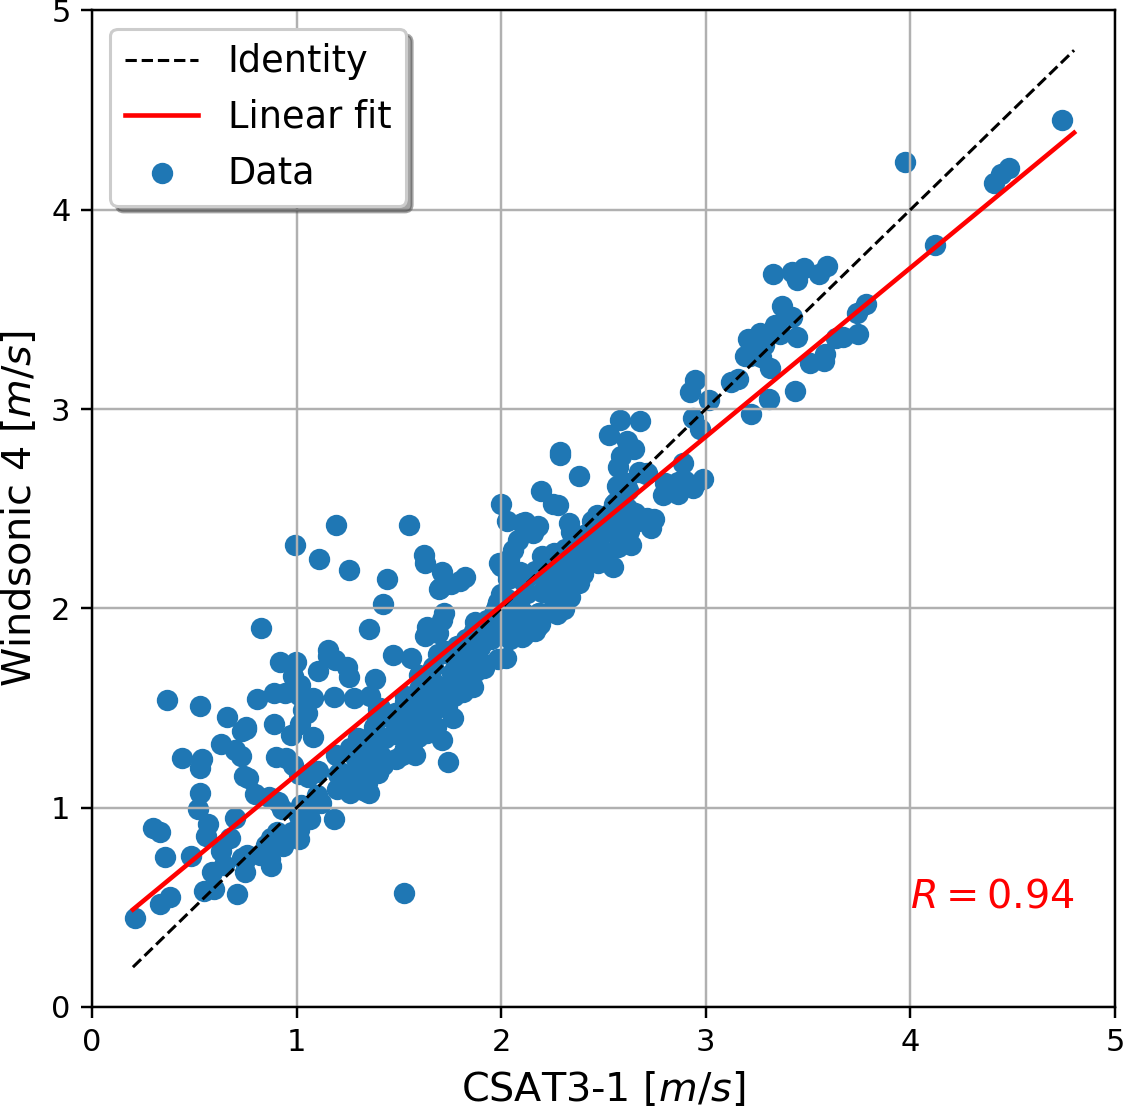
\includegraphics[width=0.48\textwidth]{fig/chapter_4/gunshot_csat1_vs_ws3.png}
    \caption{Scatter plot comparing the wind speeds of the Windsonic 4 and the CSAT3 No.1. The red line is a linear fit done to the data, with a correlation coefficient $R$ of 0.94.}
    \label{fig:csat1_vs_ws3}
\end{figure}

Figure~\ref{fig:csat_vs_TC} shows the comparison of the temperature measured with the CSAT3 and the Thermocouples. In particular, the figure on the left is the comparison between the CSAT3-B and the thermocouple 1, which are the instruments closest to the ground. It's correlation coefficient is $R = 0.996$. On the right side, the figure compares the CSAT3 No.4 with the Thermocouple 6. The data had a correlation coefficient $R = 0.989$. Thus the sensors seem reliable to measure the temperature.

In overall, the CSAT3 anemometers seem to perform good measurements of temperature compared to the Thermocouples and the Windsonic 2-D measurements are congruent with the wind speed measured by the CSAT3 anemometers.

\begin{figure}[!ht]
    \centering
    \begin{subfigure}[b]{0.48\textwidth}
        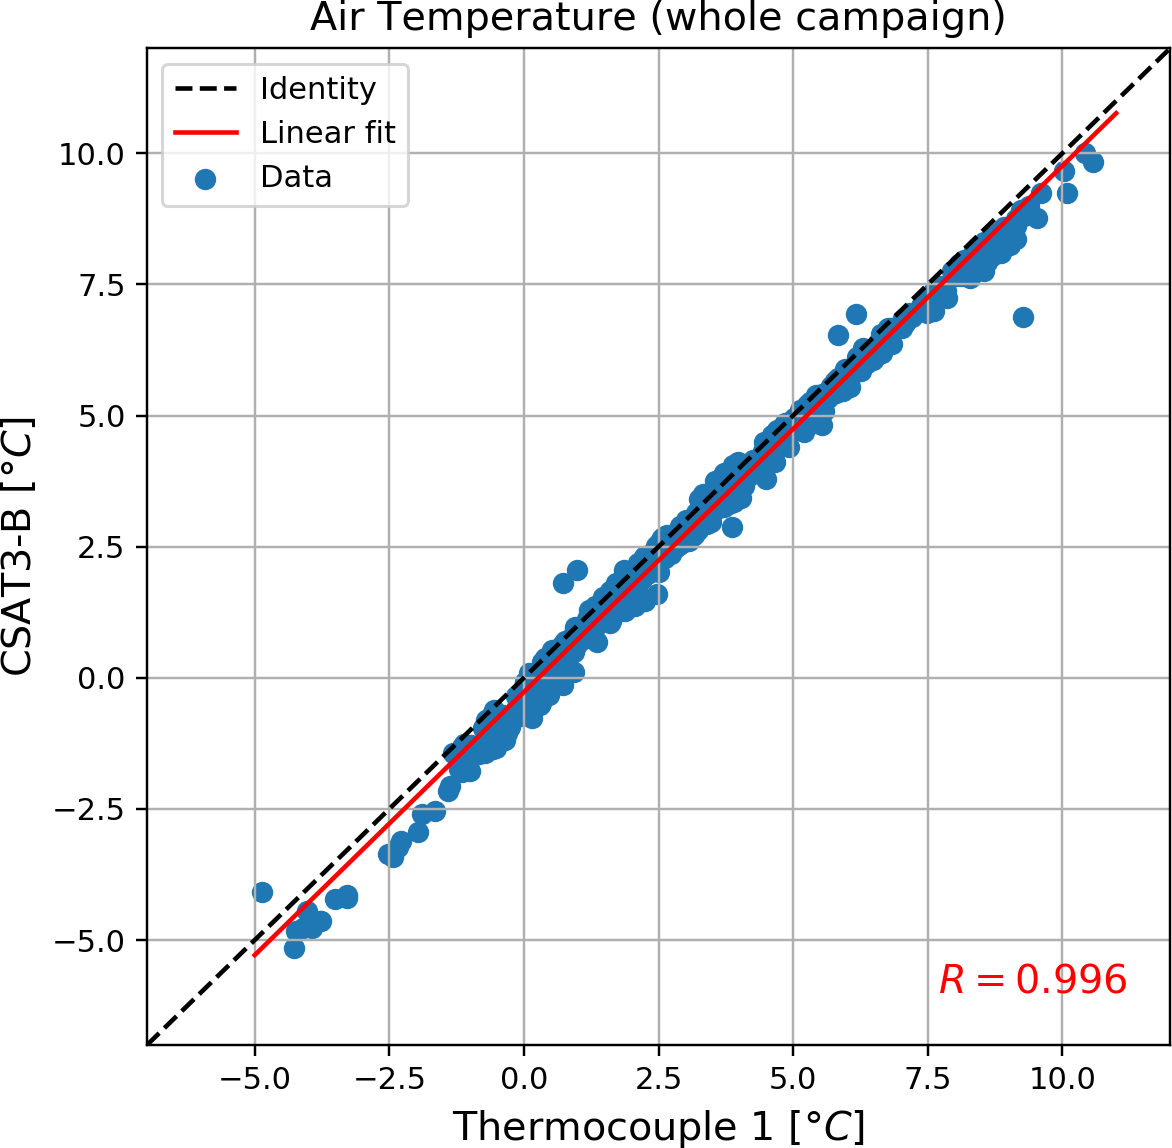
\includegraphics[width=\textwidth]{fig/chapter_4/csat3b_vs_T1.png}
      \label{fig:csat3b_vs_TC1}
    \end{subfigure}
    \quad
    \begin{subfigure}[b]{0.48\textwidth}
        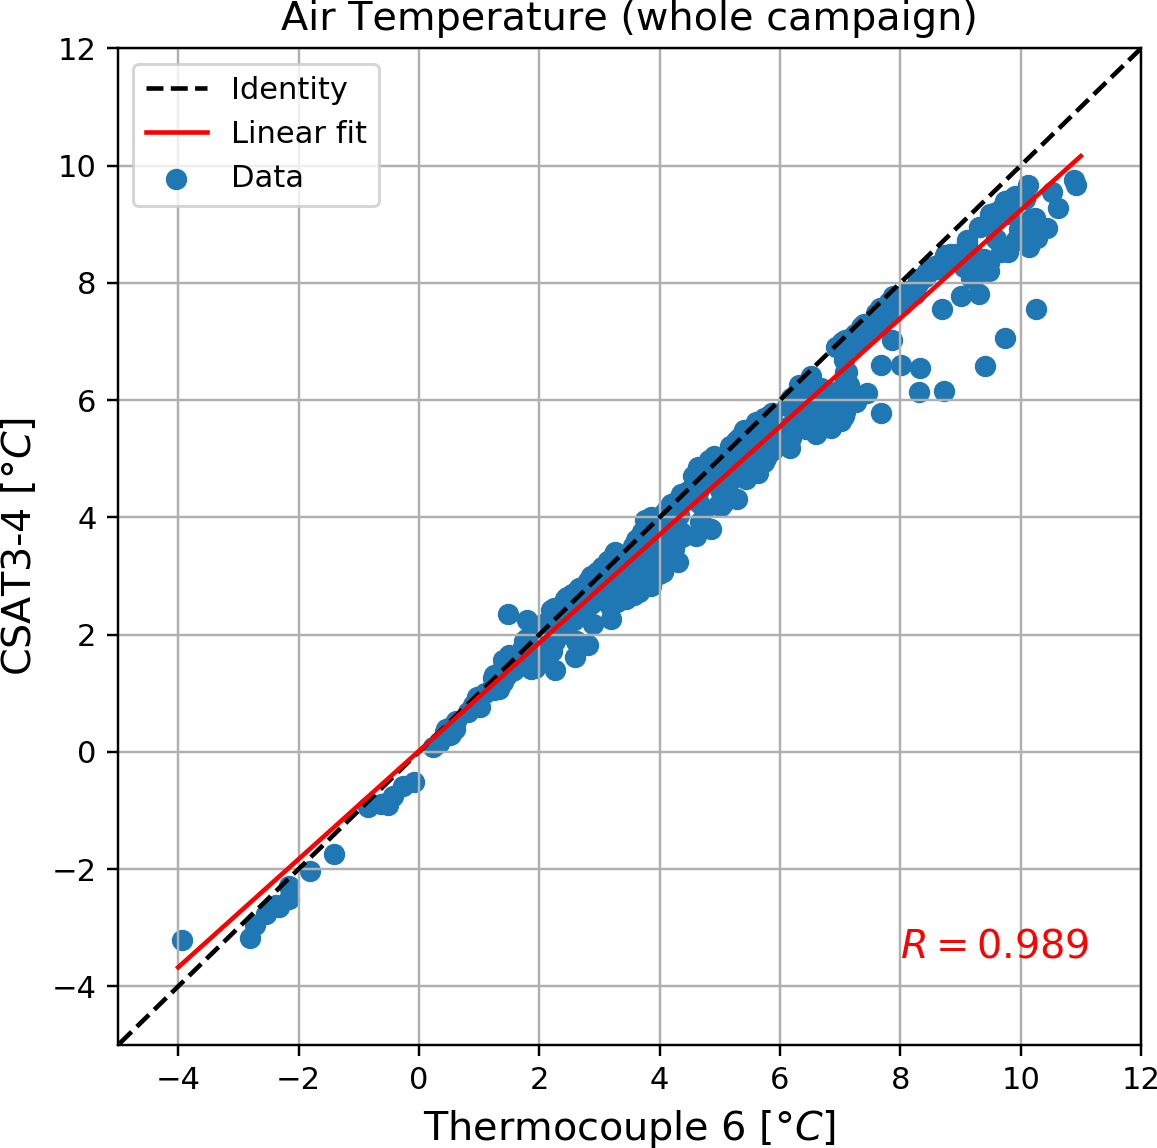
\includegraphics[width=\textwidth]{fig/chapter_4/csat4_vs_T6.png}
        \label{fig:csat4_vs_TC6}
    \end{subfigure}
    \caption{Comparison between the sonic temperature measured with the CSAT3 instruments with a Thermocouple placed at the same vertical level. Each plot has a correlation coefficient, $R$.}
    \label{fig:csat_vs_TC}
\end{figure}

%\section{Temperature gradient}

%Pending (probably not going to put it).

\section{Temperature and wind speed vertical profiles}

For sake of simplicity and because the nights of the 16-17th and 23-24th are similar, in this section we present only the 23-24th night, leaving the results of the 16-17th night for the appendix~\ref{app:profiles}. 

%\subsection{Night of the 23th to the 24th}

\begin{figure}[!ht]
    \centering
    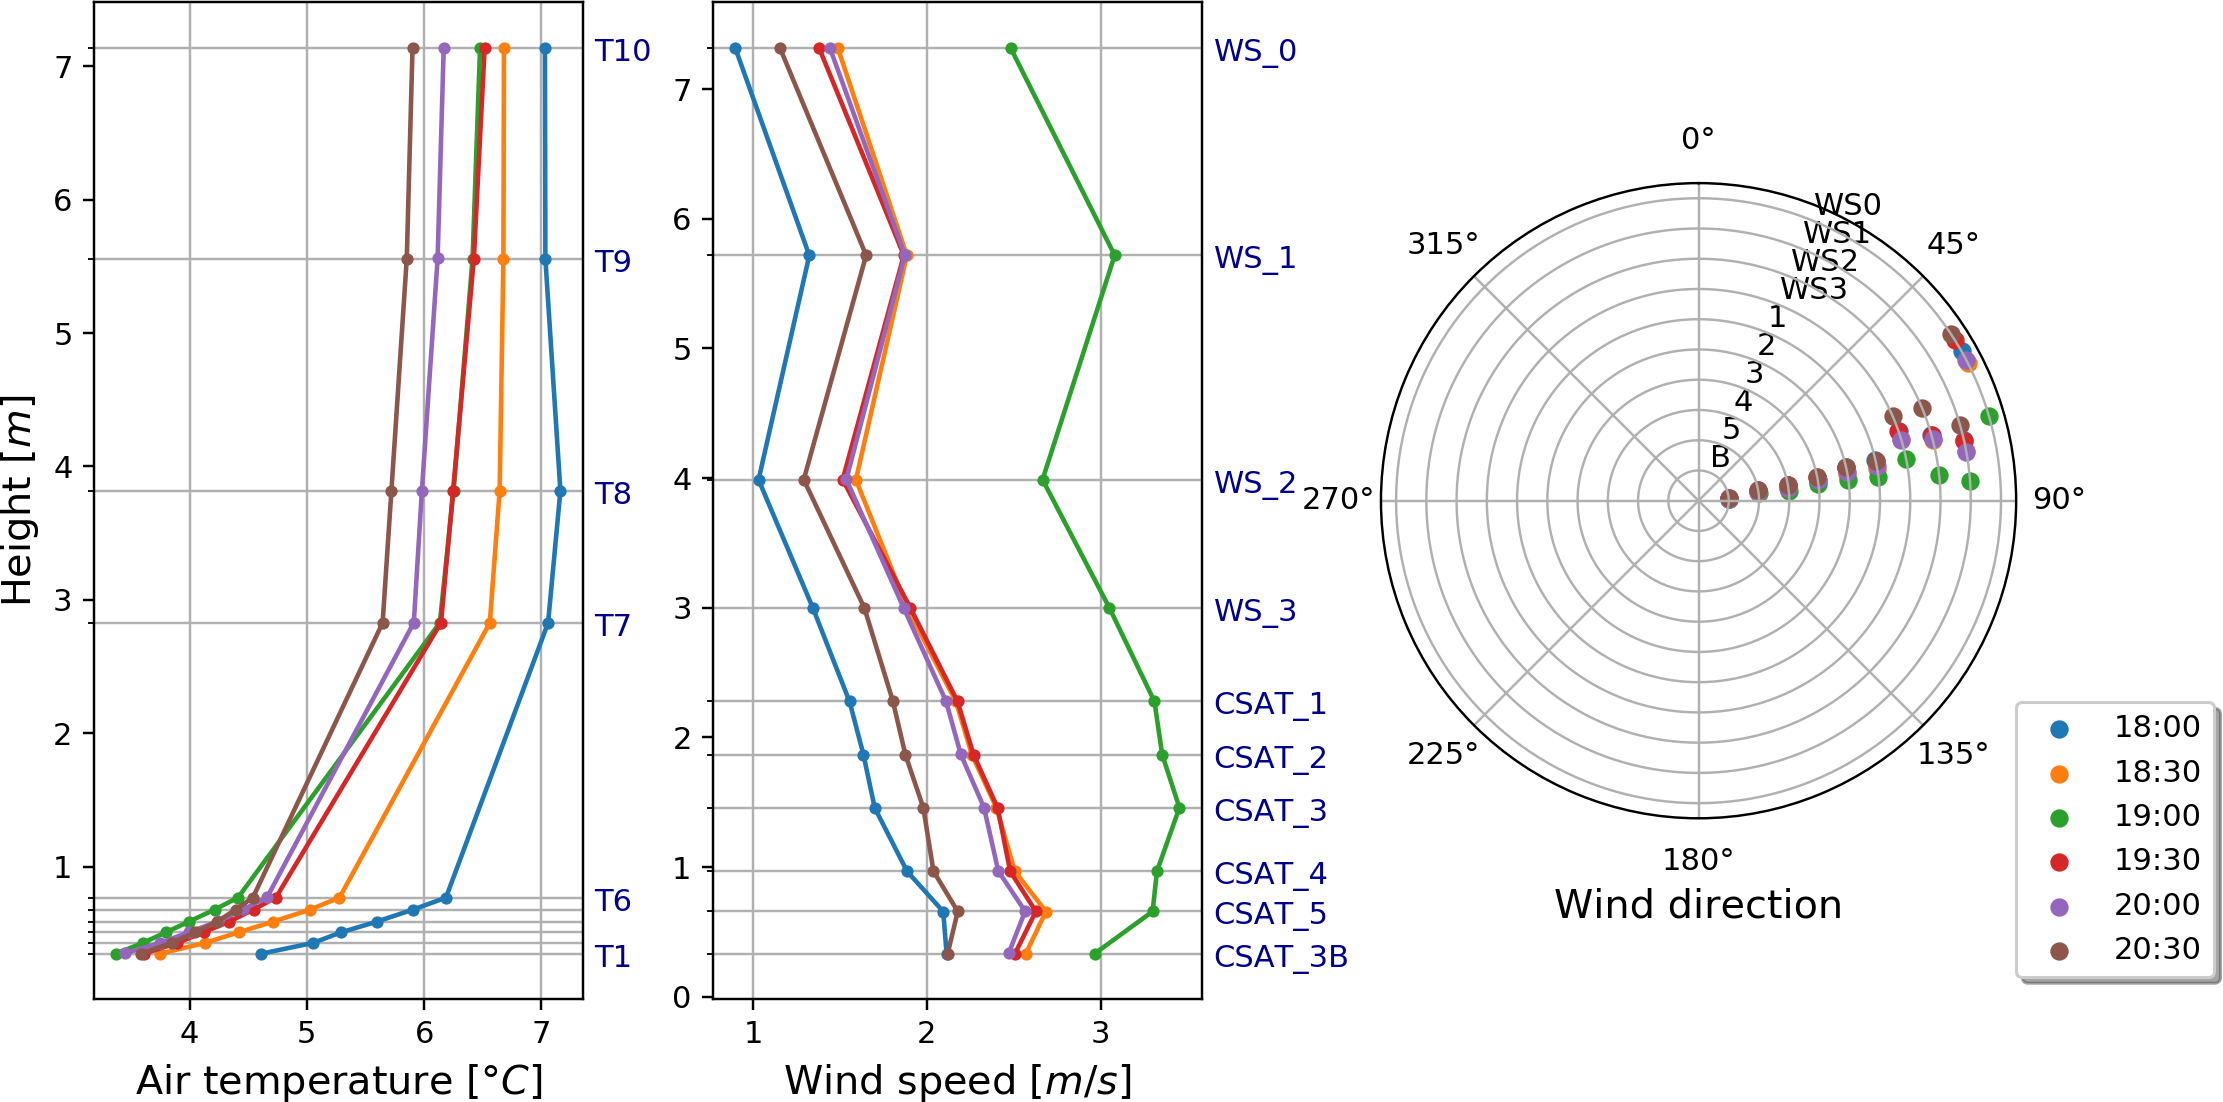
\includegraphics[width=1\textwidth]{fig/chapter_4/23-24/18-21_profiles.png}
    \caption{Temperature and wind speed vertical profiles, with the corresponding wind direction at a particular time, for the period between 18h00 and 20h30 on the night of the 23-24th.}
    \label{fig:18-21_profiles.png}
\end{figure}

Figure~\ref{fig:18-21_profiles.png} shows the vertical mean profiles of air temperature and wind speed over a period between 18h00 and 20h30. The air temperature profiles show the measurements done using the Thermocouples (T1 - T10). The wind speed profiles show the measurements done by the CSAT3 and Windsonic 2-D anemometers. At the right of the figure is possible to see a polar plot with the wind direction (point into the direction where the wind is coming to the instrument). The $0 \degree$ angle is aligned with the North. Each level of different radius corresponds to the value of a certain instrument: closer to the centre is the CSAT3-B (B), and in the outer radius, the Windsonic 2-D No.0 (WS0). Globally, the colour of the curves and points on the three subfigures correspond to the values at the same hour, which allows us to identify the temperature, the wind speed and the direction of the profile at a particular time.

\begin{figure}[!ht]
    \centering
    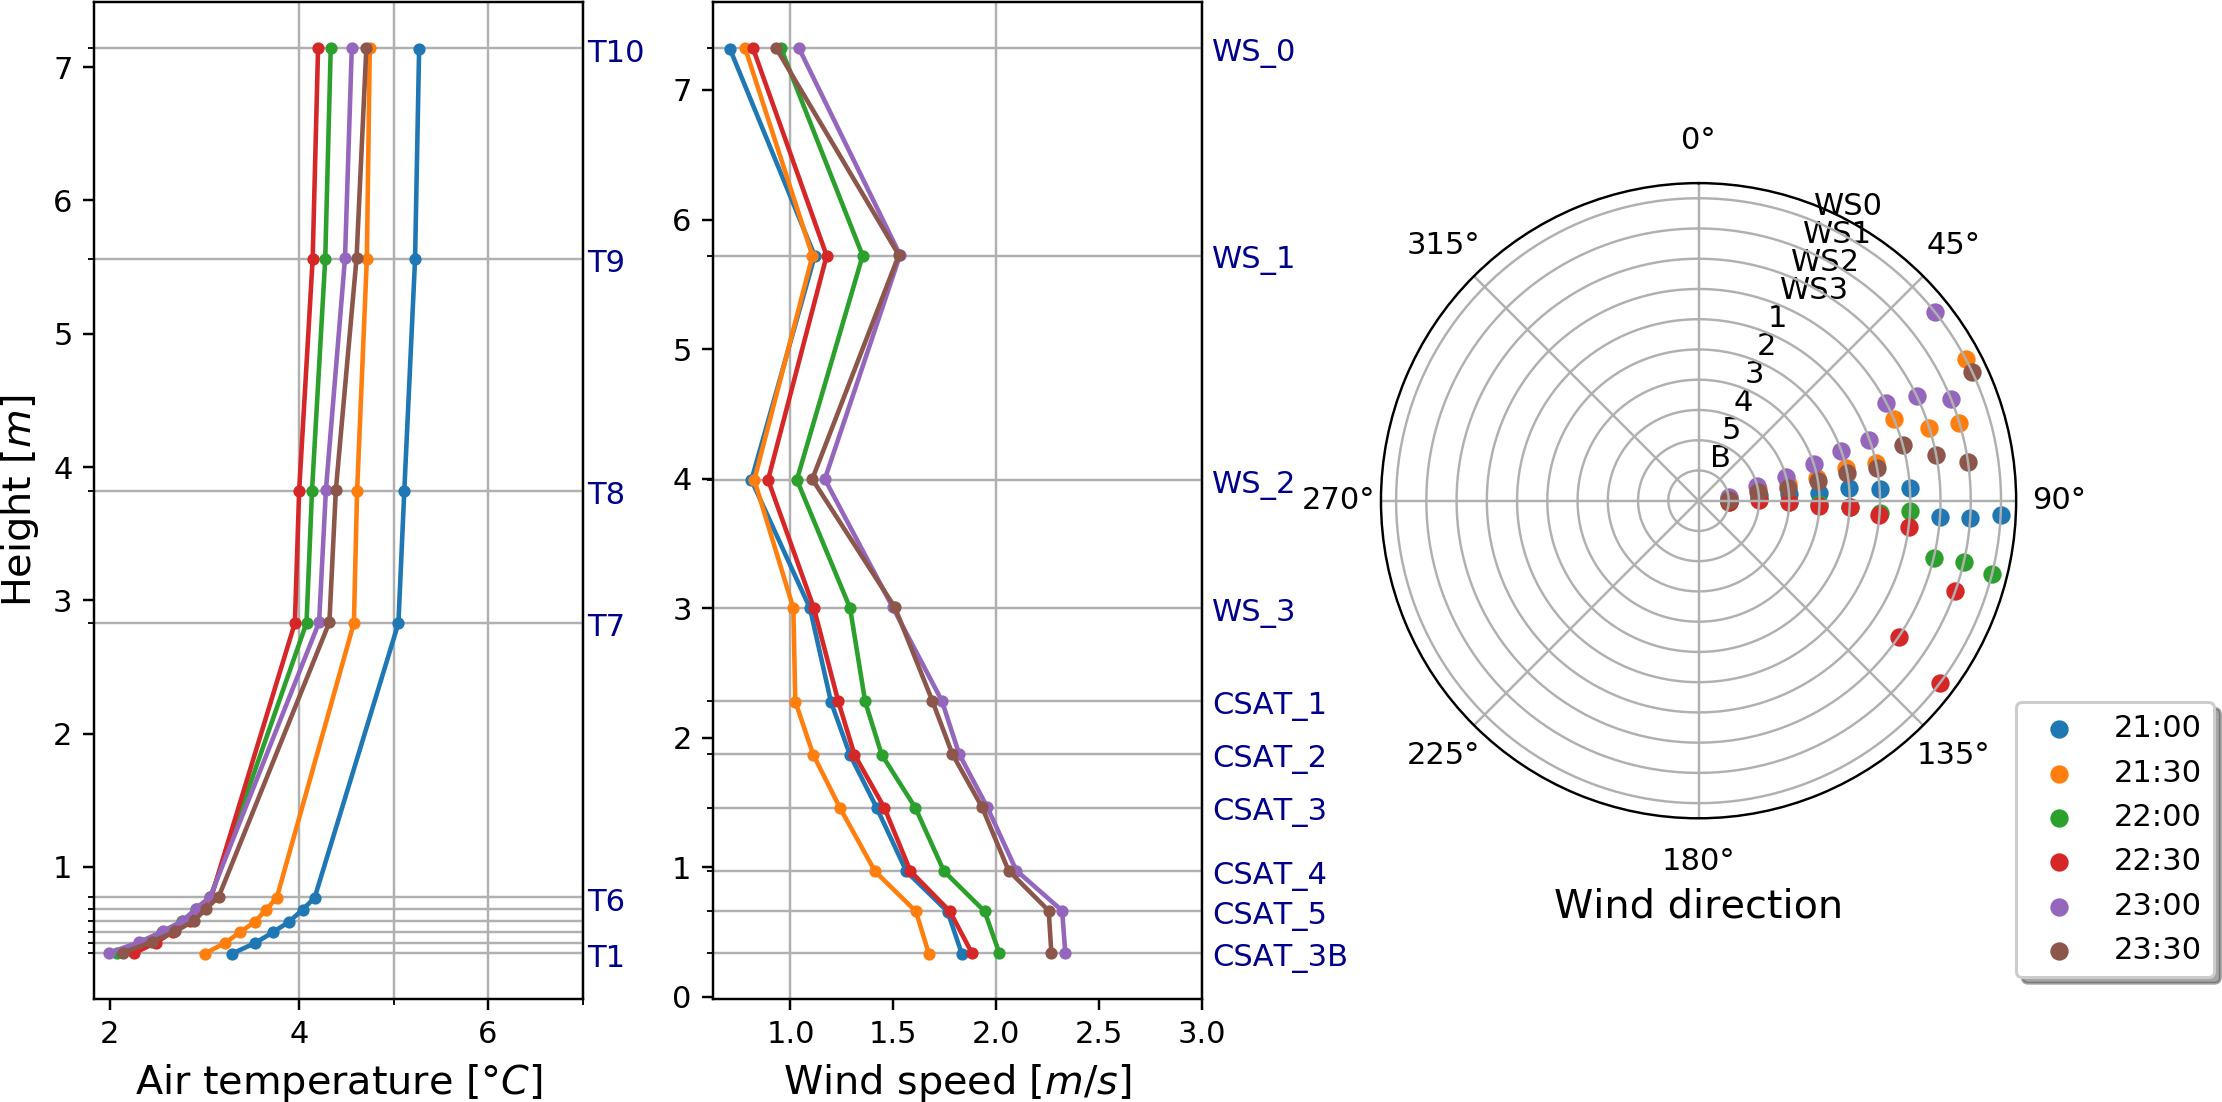
\includegraphics[width=1\textwidth]{fig/chapter_4/23-24/21-23_profiles.png}
    \caption{Temperature and wind speed vertical profiles, with the corresponding wind direction at a particular time, for the period between 21h00 and 23h30 on the night of the 23-24th.}
    \label{fig:21-23_profiles.png}
\end{figure}

Similar to the previous figure, figure~\ref{fig:21-23_profiles.png} shows the vertical profiles of air temperature and wind speed for the period between 21h00 and 23:30, with the corresponding wind direction.

The figures~\ref{fig:18-21_profiles.png} and \ref{fig:21-23_profiles.png} show typical profiles of katabatic wind, characterised by having a low
wind speed with a maximum close to the surface, inside a stable environment where temperature increases with height. Also, in the period shown in both figures, we can see a persistent wind direction coming from the downslope direction, especially in the lower levels. This confirms that during this night there were katabatic winds coming down the slope of the mountain. 

\section{Vertical fluxes and TKE}

In this section, we present the momentum flux ($\tau$), the sensible heat flux ($H$) and the Turbulent Kinematic Energy (TKE), computed with a five minutes average for the night of the 23-24th of February. As in the previous section, the fluxes for the night of the 16-17th can be found in the appendix~\ref{app:profiles}.

\begin{figure}[!ht]
    \centering
    \begin{subfigure}[b]{0.58\textwidth}
        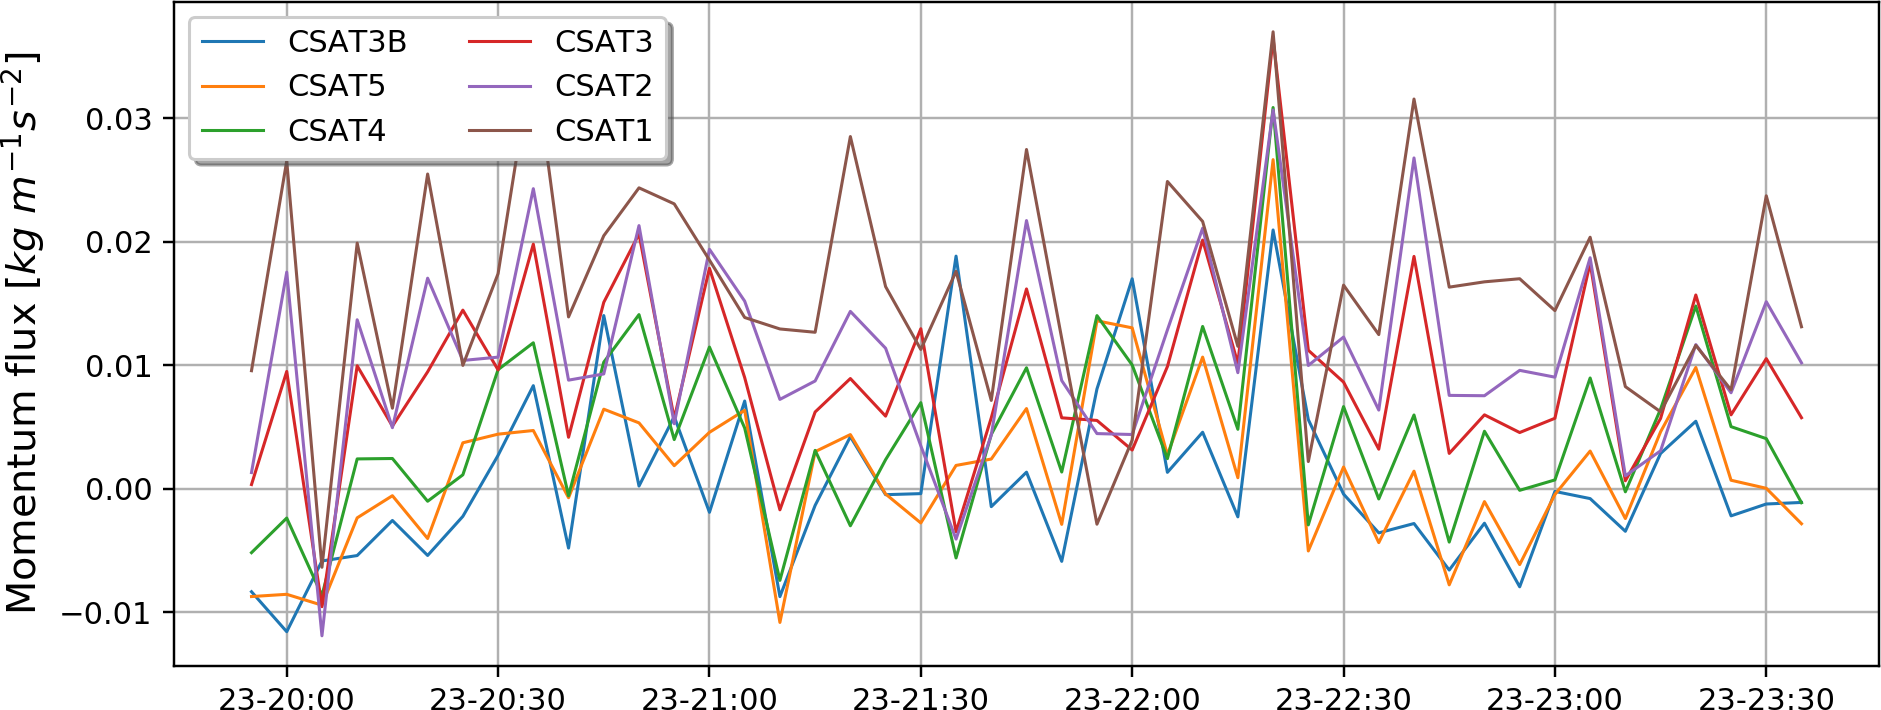
\includegraphics[width=\textwidth]{fig/chapter_4/23-24/Tau_23-24.png}
      \label{fig:Tau_23-24}
    \end{subfigure}
    \begin{subfigure}[b]{0.58\textwidth}
        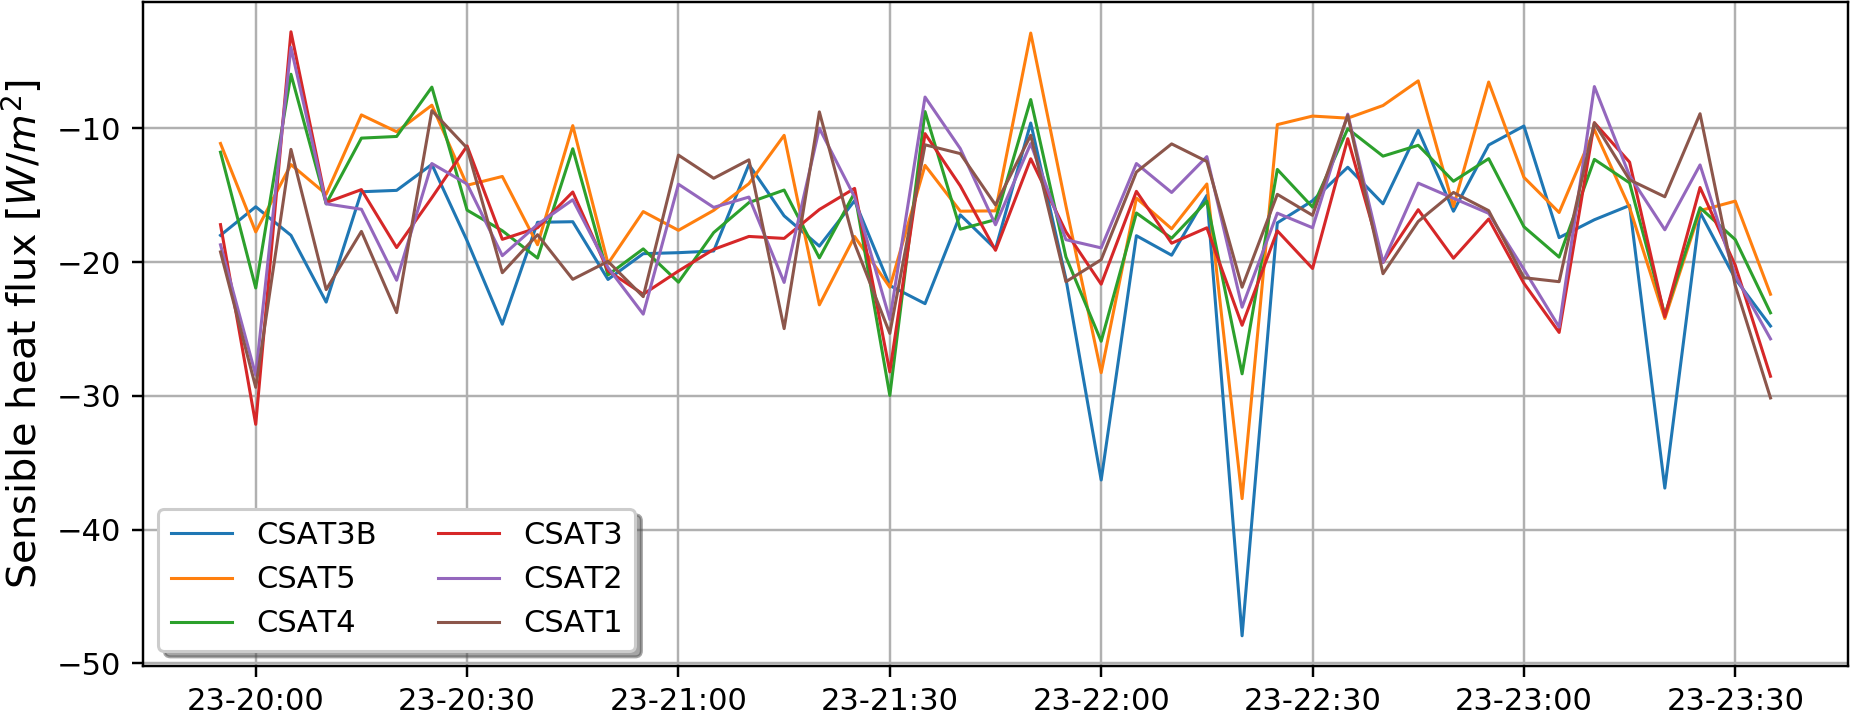
\includegraphics[width=\textwidth]{fig/chapter_4/23-24/H23-24.png}
        \label{fig:H_23-24}
    \end{subfigure}
    \begin{subfigure}[b]{0.58\textwidth}
        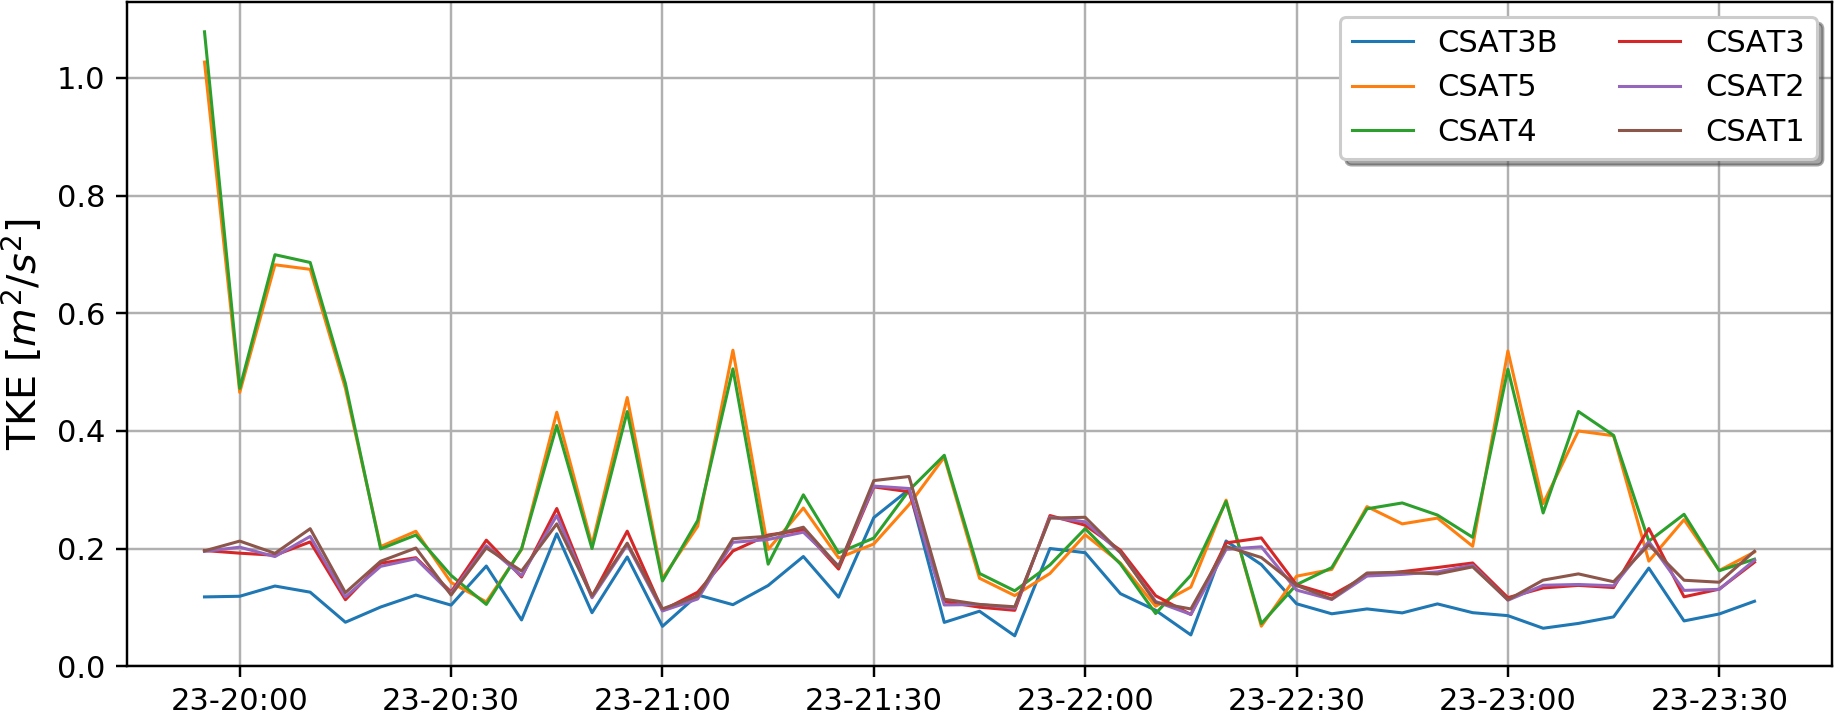
\includegraphics[width=\textwidth]{fig/chapter_4/23-24/TKE23-24.png}
        \label{fig:TKE_23-24}
    \end{subfigure}
    \caption{Time series of the momentum flux (upper figure), temperature flux (middle figure) and Turbulent Kinetic Energy (lower figure). }
    \label{fig:23-24_flux_series}
\end{figure}

Figure~\ref{fig:23-24_flux_series} shows the time series from the three fluxes between the 20h00 up to 23h30. These fluxes are only shown for the CSAT3 anemometers, and that is because these instruments measure simultaneously the temperature and the three components of the wind, making them the only anemometers to be able to compute these variables. The time series shows the variation of these quantities over time but is difficult to identify the value that corresponds to a particular instrument, for that it is useful to plot vertical profiles.

To improve the analysis we selected a particular hour, based on the 30 minutes average profiles, that had a clearly defined maximum wind speed and with a wind direction coming from $90\degree$ upslope. With this in mind, we selected two hours during the night and plotted the vertical profiles. The selected times were 20h00 and 23h00. Figure~\ref{fig:vert_prof_a} shows four profiles around 20h00, where at the left is the momentum flux ($\tau$), the second panel corresponds to the sensible heat flux ($H$), the third is the Turbulent Kinetic Energy (TKE) and the fourth one is the wind speed profile ($u$). In the same manner, figure~\ref{fig:vert_prof_b} shows the profiles for the fluxes, the TKE and the wind speed around 23h00. 

\begin{figure}
    \centering
    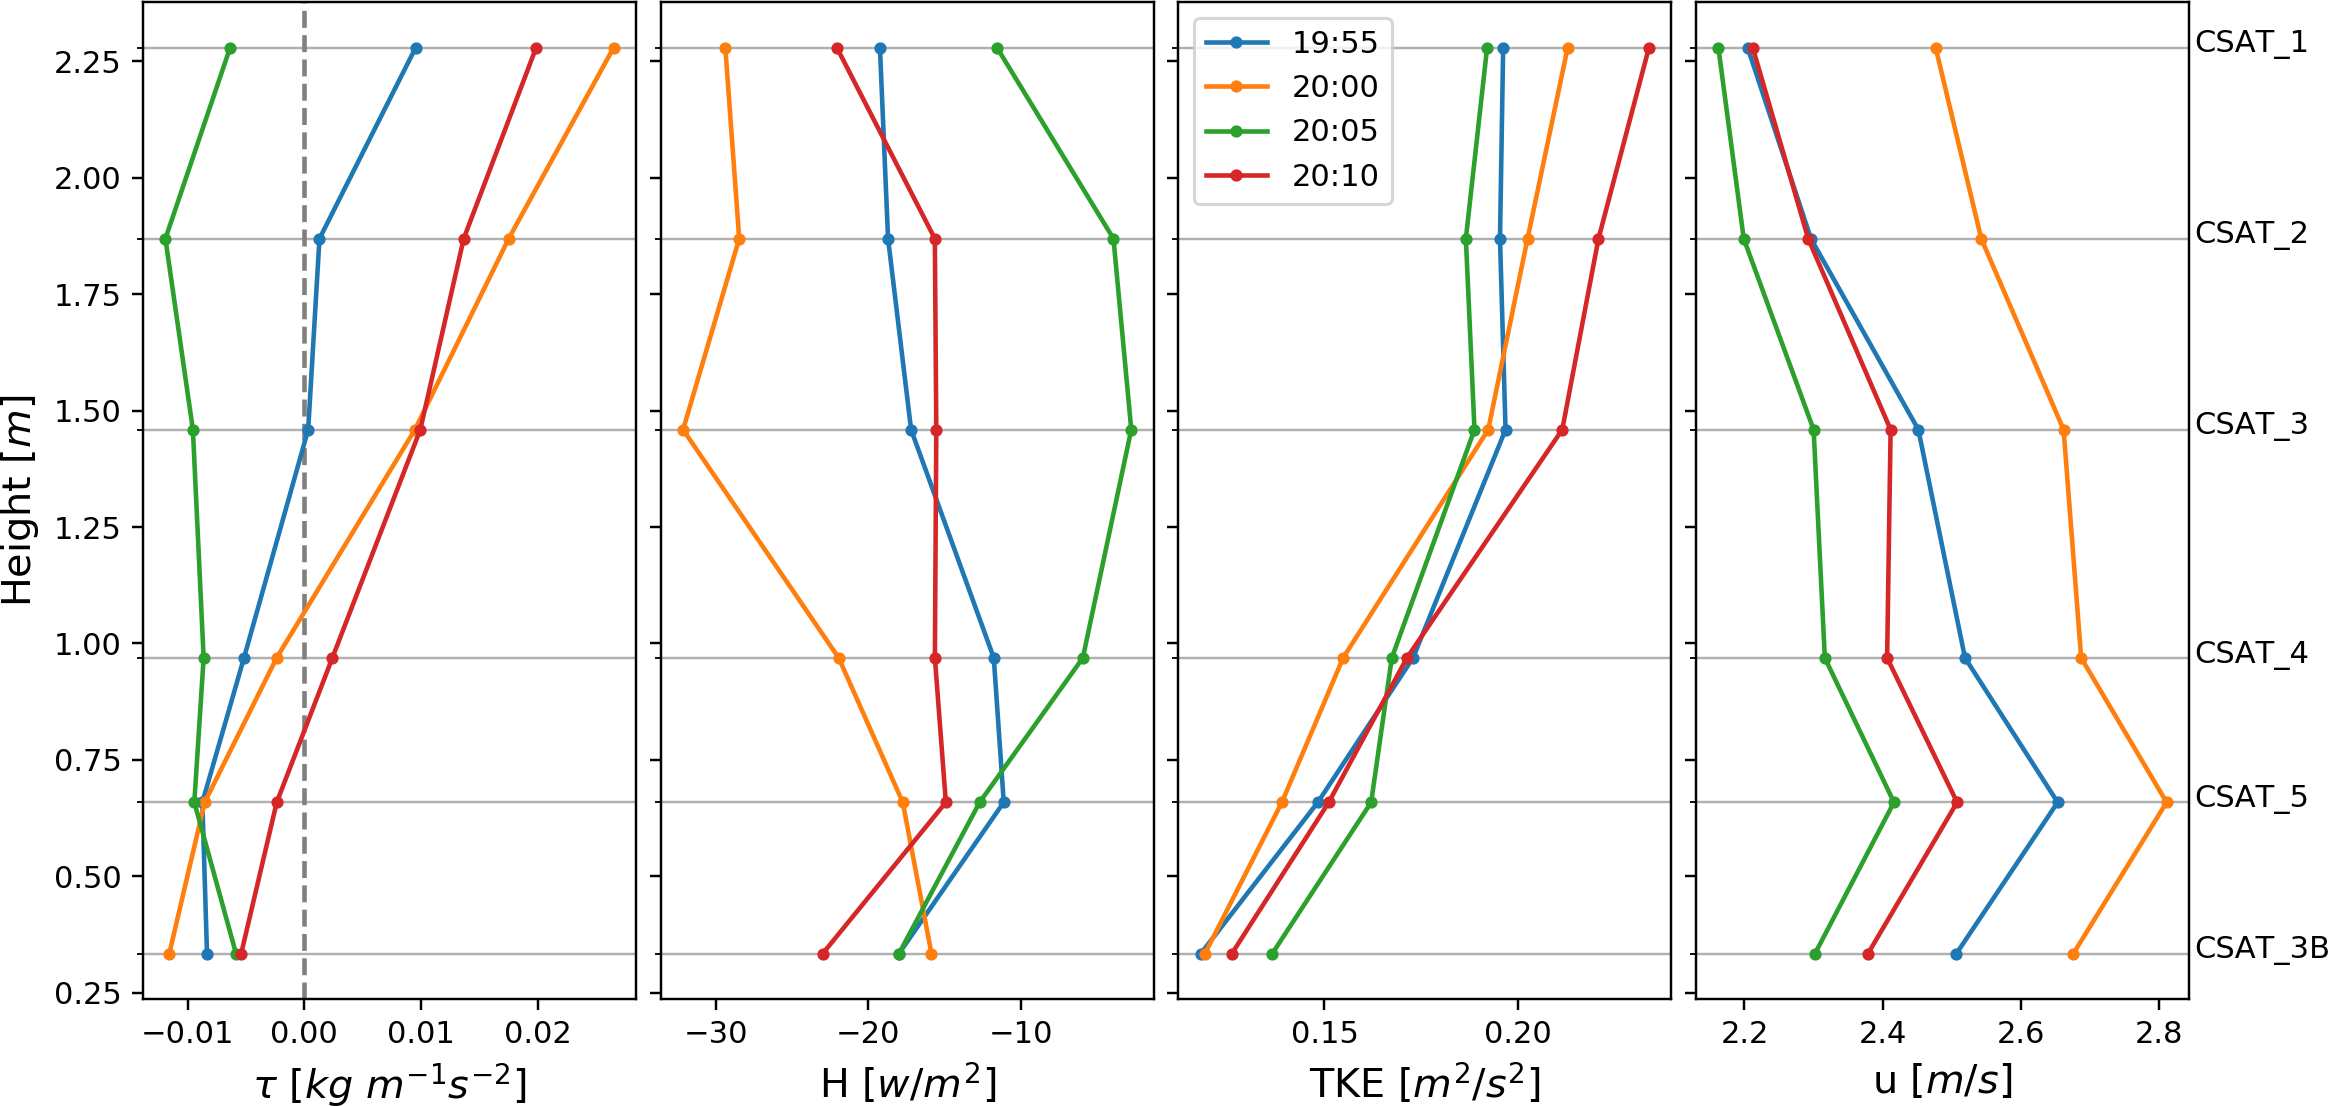
\includegraphics[width=1\textwidth]{fig/chapter_4/23-24/vert_prof_a_speedmax.png}
    \caption{Vertical profiles of momentum flux ($\tau$), sensible heat flux ($H$), Turbulent Kinetic Energy (TKE) and wind speed ($u$), for the night of the 23-24th of February, around 23h00.}
    \label{fig:vert_prof_a}
\end{figure}

Figure~\ref{fig:vert_prof_a} shows that the wind speed maximum is located at the same level as the CSAT3 No. 5, i.e. between 0.5m and 0.75m. In theory, the momentum flux at the maximum has to be equal to zero, which is the case of the profile corresponding to 20h10. For the other profiles, we see that the zero in the momentum flux is higher, at 1m or more. And at 19h55, we see that the momentum flux is always negative. As well, we can see that $\tau$ is strong in magnitude close to the surface due to strong shear stress caused by friction. 

\begin{figure}[!ht]
    \centering
    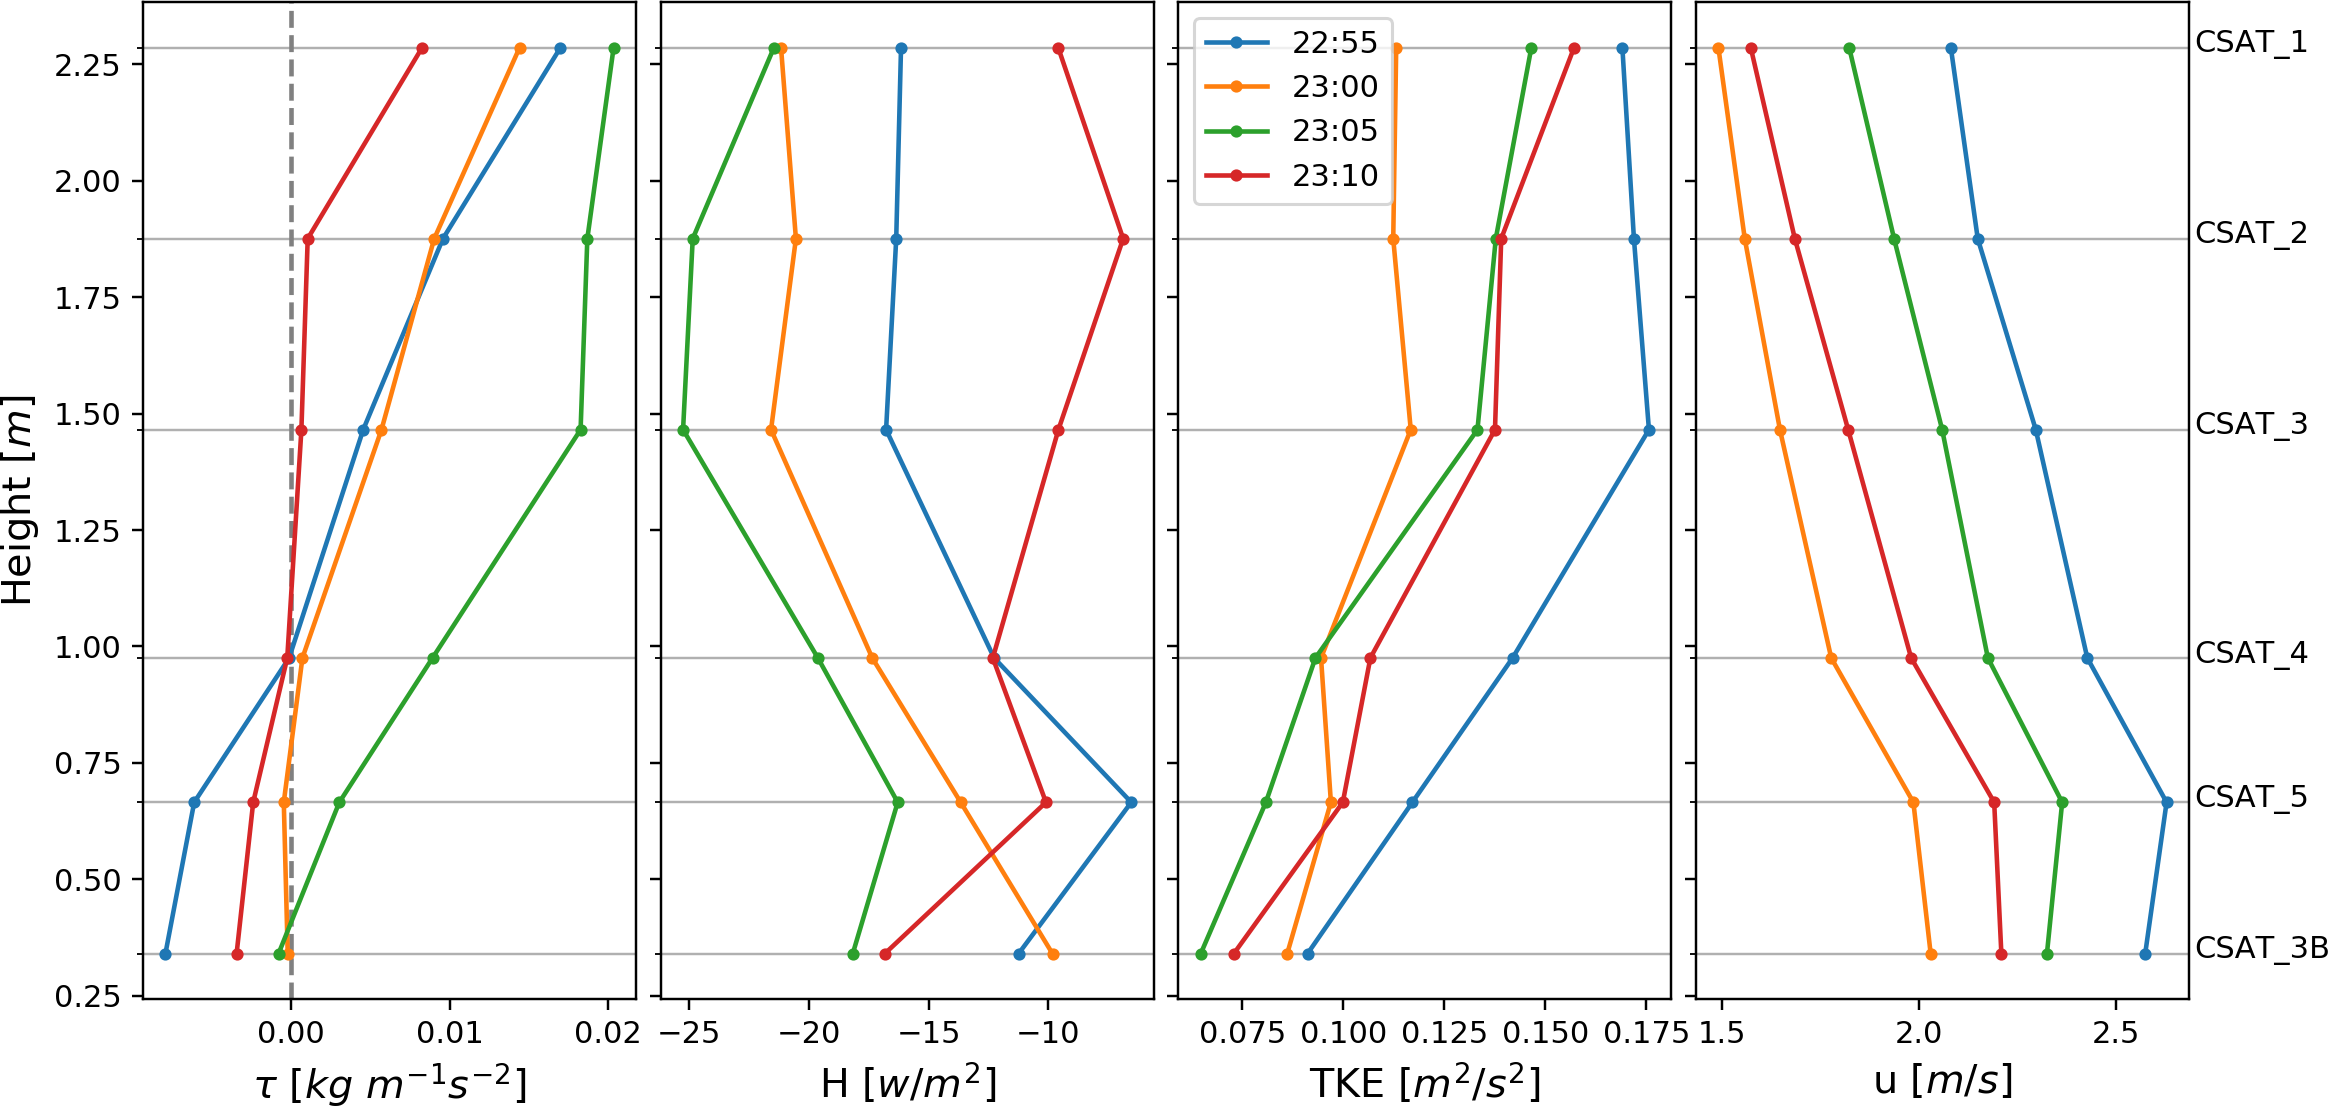
\includegraphics[width=1\textwidth]{fig/chapter_4/23-24/vert_prof_b_speedmax.png}
    \caption{Vertical profiles of momentum flux ($\tau$), sensible heat flux ($H$), Turbulent Kinetic Energy (TKE) and wind speed ($u$), for the night of the 23-24th of February, around 23h00.}
    \label{fig:vert_prof_b}
\end{figure}

Regarding the sensible heat flux ($H$) on figure~\ref{fig:vert_prof_a}, we see that it is always negative for all the profiles. This is due to the stable environment where the air is colder in the lower layers. The vertical profiles were expected to be constant with height, but the profiles show variations, which are difficult to explain. Concerning the Turbulent Kinetic Energy, it is small close to the surface due to the strong stability of the layer because is related to a strong temperature gradient. In the upper levels, the TKE is large due to the large shear stress and a smaller temperature gradient.

Finally, figure~\ref{fig:vert_prof_b} shows the vertical profiles corresponding to 23h00. In a similar way than the previous figure, The mean wind maximum is located at the level of the CSAT3 No.5. The momentum flux is negative for the lower part of the profile, below the maximum, and is positive above the maximum. The Sensible heat flux remains negative as expected (stable profile), but there are still some variations that are difficult to explain. For the TKE, we see that the profiles are similar to the ones in figures~\ref{fig:vert_prof_a}, with the lower value at the lower layer, and a larger one above the wind maximum.